\documentclass[conference,a4paper]{IEEEtran}
\usepackage{fontspec}
\setmainfont{Liberation Serif}
\setsansfont{Carlito}
\setmonofont{DejaVu Sans Mono}[Scale=0.85]
\usepackage[spanish,es-tabla,es-nodecimaldot]{babel}
\usepackage{graphicx,booktabs,array,xcolor,tikz}
\usetikzlibrary{arrows.meta,positioning}
\usepackage{cite}
\usepackage[hidelinks]{hyperref}
\usepackage{url}
\newcolumntype{L}[1]{>{\raggedright\arraybackslash}p{#1}}
% generado por pruebas/conftest.py: no editar a mano
\newcommand{\PruebasOk}{77}
\newcommand{\PruebasTotal}{81}
\newcommand{\PruebasFallan}{4}

\newcommand{\Repo}{https://github.com/angelrampolo/proyecto-interciclo-rvh}
\newcommand{\Tag}{v1.0-entrega}
\newcommand{\sint}{\textit{(datos sintéticos, SUMO)}}
\graphicspath{{figuras/}}
\definecolor{ia}{HTML}{0F8F7F}
\definecolor{mal}{HTML}{C0392B}
\newcommand{\ok}{\textcolor{ia}{\textbf{cumple}}}
\newcommand{\no}{\textcolor{mal}{\textbf{no cumple}}}

\begin{document}

\title{Centro de tráfico predictivo para Cuenca: predicción de velocidad a una hora, detección automática de incidentes y aviso V2X validado en bucle cerrado con SUMO}

\author{\IEEEauthorblockN{Angel Apolo, Fernando Terán, Stalyn Ochoa y Karla Barrera}
\IEEEauthorblockA{Facultad de Ingeniería, Universidad de Cuenca\\
Redes Vehiculares, Proyecto Interciclo\\
Cuenca, Ecuador}}

\maketitle

\begin{abstract}
Cuando un accidente cierra una avenida, el centro de tráfico suele enterarse cuando la cola ya creció y los vehículos que vienen detrás siguen entrando a ella. Este trabajo cierra el lazo dato--modelo--acción--medida--visualización para Cuenca sobre un gemelo digital en SUMO con datos sintéticos justificados. Un modelo GCN-GRU predice la velocidad de las 1694 celdas de 200~m de la ciudad a 60~min como corrección del promedio histórico; un detector automático de incidentes (AID) basado en \emph{gradient boosting} vigila tres corredores minuto a minuto; y, en bucle cerrado mediante TraCI, una alarma confirmada genera un mensaje DENM para los vehículos conectados cercanos, que recalculan su ruta. Cada parte se compara con una línea base justa y se verifica con un banco de \PruebasTotal{} pruebas automáticas. En el test, el error medio a 60~min es de 1,82~km/h con sensores y 1,86~km/h con solo el 50~\% de vehículos V2X, frente a 3,16~km/h del promedio histórico. El AID detecta el 90~\% de los incidentes que forman cola en 4,5~min (14~\% un detector al azar con la misma tasa de falsas alarmas), con 1,9--4,4~\% de falsas alarmas. En SUMO, el aviso reduce en 27,8~\% la demora de los vehículos afectados por un cierre total y en 8,1~\% la de toda la red. Todos los resultados son sintéticos y el código acepta datos reales con el mismo formato.
\end{abstract}

\begin{IEEEkeywords}
V2X, DENM, SUMO, TraCI, redes neuronales de grafos, GRU, detección automática de incidentes, gemelo digital, datos sintéticos.
\end{IEEEkeywords}

\section{Introducción}
Un centro de control de tráfico necesita responder tres preguntas: cómo estará la ciudad dentro de un rato, dónde acaba de ocurrir un incidente y qué hacer para que afecte a la menor cantidad de conductores. La comunicación vehicular (V2X) agrega una fuente de datos, los vehículos conectados, y un canal de actuación, los mensajes de aviso como el DENM del estándar ETSI~\cite{etsi_denm}.

El objetivo fue construir y evaluar ese ciclo completo sobre la red real de Cuenca: (i) predecir la velocidad de toda la ciudad a 1~h con un error medio menor a 3~km/h; (ii) detectar incidentes en tres corredores con una tasa de detección (DR) de al menos 85~\%, un tiempo medio de detección (MTTD) menor a 5~min y una tasa de falsas alarmas (FAR) de 3--5~\%; y (iii) demostrar en simulación que el aviso V2X reduce las demoras. Como los datos de la EMOV EP no estaban disponibles para el periodo de estudio, el trabajo usa datos sintéticos generados en SUMO~\cite{sumo}, justificados en el Anexo y etiquetados como tales en cada tabla y figura.

Las contribuciones son: un predictor liviano que aprende la corrección sobre lo habitual y funciona con sensores y con datos V2X parciales; un detector evaluado siempre frente a un detector al azar con la misma tasa de alarmas; una validación en bucle cerrado real en SUMO, con y sin la IA sobre el mismo día; y un repositorio que repite el experimento completo con un solo script (Sección~\ref{sec:replica}).

\section{Estado del arte}\label{sec:arte}
Revisamos siete trabajos recientes en tres líneas: predicción con redes de grafos, detección automática de incidentes y avisos V2X evaluados en simulación. La Tabla~\ref{tab:arte} los compara con nuestra propuesta.

\textbf{Predicción espaciotemporal con grafos.} T-GCN~\cite{zhao2020tgcn} combina una convolución de grafo con una GRU para predecir la velocidad en carreteras urbanas de Shenzhen y en autopistas de Los Ángeles. Es la base de nuestra arquitectura.
\begin{itemize}
\item \textbf{Graph WaveNet}~\cite{wu2019graphwavenet}: parte de que el grafo dado puede no reflejar las dependencias reales entre sensores. Aprende una matriz de adyacencia adaptativa y la combina con convoluciones temporales dilatadas. En METR-LA y PEMS-BAY, con autopistas y lazos reales, obtiene a 60~min un MAE de 3,53 y 1,95~mph.
\item \textbf{GMAN}~\cite{zheng2020gman}: ataca la degradación de la predicción a 1~h con un codificador-decodificador de atención espacial y temporal. Alcanza un MAE de 1,86~mph a 60~min en PeMS-BAY, frente a 3,38~mph de ARIMA.
\item \textbf{Revisión de Jiang y Luo}~\cite{jiang2022gnnsurvey}: ordena más de un centenar de trabajos de GNN para tráfico y muestra que casi todos los benchmarks son autopistas de EE.~UU. y China.
\end{itemize}
Estos modelos predicen la velocidad absoluta con datos reales y no actúan sobre el tráfico. Nosotros predecimos la corrección sobre el promedio histórico en una red urbana sintética, con datos V2X parciales, y usamos la predicción dentro de un lazo. Sus errores están en mph y sobre otras redes, así que no son comparables con nuestros km/h.

\textbf{Detección automática de incidentes.}
\begin{itemize}
\item \textbf{Sun et al.}~\cite{sun2022weakaid}: notan que las etiquetas de incidentes de PeMS tienen errores de hora y lugar, y las limpian con supervisión débil antes de entrenar bosques aleatorios, SVM y LSTM. En la I-80 logran DR~0,90 y FAR~0,08, pero su FAR es la fracción de alarmas que son falsas, no la fracción de intervalos sin incidente que tienen alarma, como en nuestro caso.
\item \textbf{Parsa et al.}~\cite{parsa2020xgboost}: usan XGBoost, la misma familia que nuestro clasificador, con variables de tráfico, red y clima, y SHAP para interpretarlo. En autopistas de Chicago reportan DR~79~\% y FAR~0,16~\%.
\end{itemize}
Ninguno de los dos compara contra un detector al azar con la misma tasa de alarmas, ni trabaja en arterias urbanas con firma aguas arriba y aguas abajo, contexto de red y lluvia. Las cifras de AID dependen mucho de cómo se define la FAR, y por eso damos la nuestra de forma explícita.

\textbf{Avisos V2X evaluados en SUMO.}
\begin{itemize}
\item \textbf{Porfyri et al.}~\cite{porfyri2019rhw}: evalúan un aviso de peligro V2I en SUMO con TraCI sobre una autopista de 5~km y penetraciones de 0 a 100~\%. Los vehículos avisados reducen su velocidad y amplían su distancia, lo que baja los choques simulados. El incidente se conoce de antemano y no hay cambio de ruta.
\item \textbf{ms-van3t}~\cite{raviglione2024msvan3t}: integra la pila ETSI completa (CAM, DENM) sobre ns-3 acoplado a SUMO para validar servicios V2X con varias tecnologías de acceso. Es la base de VaN3Twin~\cite{pegurri2026van3twin}, la plataforma del curso.
\end{itemize}
Ninguno acopla un detector automático ni mide el beneficio de un cambio de ruta disparado por DENM en una red urbana. Nuestro DENM se emula a nivel de aplicación con TraCI, con comunicación ideal; acoplarlo a la pila de radio de ms-van3t queda como trabajo futuro.

\begin{table*}[t]
\centering
\caption{Comparación de los trabajos revisados con la propuesta}
\label{tab:arte}
\scriptsize
\setlength{\tabcolsep}{3pt}
\begin{tabular}{@{}L{1.75cm}L{2.6cm}L{2.7cm}L{2.3cm}L{2.6cm}L{1.05cm}L{3.4cm}@{}}
\toprule
Trabajo & Problema & Método & Datos & Resultado & Actúa & Diferencia con este trabajo \\
\midrule
Wu et al. 2019~\cite{wu2019graphwavenet} & Predecir velocidad con grafo incompleto & Adyacencia adaptativa + convolución temporal dilatada & METR-LA, PEMS-BAY (autopistas reales) & MAE 60 min: 3,53 / 1,95 mph & No & Velocidad absoluta; no usa datos V2X parciales ni lazo cerrado \\
Zheng et al. 2020~\cite{zheng2020gman} & Predicción a largo plazo (1 h) & Atención espacial y temporal, codificador-decodificador & PeMS-BAY, Xiamen & MAE 60 min: 1,86 mph (ARIMA 3,38) & No & Modelo grande; sin lluvia ni incidentes; no actúa \\
Jiang y Luo 2022~\cite{jiang2022gnnsurvey} & Ordenar la literatura de GNN para tráfico & Revisión sistemática & Más de 100 trabajos & Taxonomía; benchmarks casi solo de autopistas & No & Casi no hay redes urbanas latinoamericanas ni V2X \\
Sun et al. 2022~\cite{sun2022weakaid} & Etiquetas de incidentes ruidosas & Supervisión débil + RF, SVM, LSTM & PeMS I-80 (real) & DR 0,90; FAR 0,08 (fracción de alarmas) & No & FAR con otra definición; sin comparar con azar; autopista \\
Parsa et al. 2020~\cite{parsa2020xgboost} & Detectar accidentes en tiempo real & XGBoost + SHAP & Autopistas de Chicago (real) & DR 79 \%; FAR 0,16 \% & No & Sin comparar con azar; casos negativos muestreados; autopista \\
Porfyri et al. 2019~\cite{porfyri2019rhw} & Impacto de un aviso de peligro V2I & SUMO + TraCI, ajuste de velocidad y distancia & Autopista sintética de 5 km & Menos choques al subir la penetración & Sí & Incidente conocido; sin detector ni cambio de ruta \\
Raviglione et al. 2024~\cite{raviglione2024msvan3t} & Validar servicios V2X sin pruebas de campo & ns-3 + SUMO con pila ETSI (CAM, DENM) & Escenarios SUMO & Interoperabilidad de la pila ETSI & Herram. & Sin predictor, sin AID y sin medir beneficio de tráfico \\
\midrule
\textbf{Este trabajo} & Prever, detectar y avisar en una ciudad & GCN-GRU residual + gradient boosting + DENM en bucle cerrado & Gemelo de Cuenca, sintético, 66 días & MAE 1,82 km/h; DR 90 \% (azar 14 \%); −27,8 \% demora & Sí & Lazo completo con líneas base justas; datos sintéticos \\
\bottomrule
\end{tabular}
\end{table*}


\section{Metodología}
\subsection{Gemelo digital y datos sintéticos}
La red vial de las 15 parroquias urbanas se obtuvo de OpenStreetMap y se convirtió con \texttt{netconvert} (16\,274 aristas, 360 semáforos). La demanda se genera como un proceso de Poisson no homogéneo con perfiles horarios distintos para laborable, sábado y domingo, origen y destino ponderados por longitud y carriles, y rutas con \texttt{duarouter}. La demanda pico se fijó en el punto de saturación de la red, V0~=~17\,000~veh/h, hallado con un barrido de tres semillas. Un día laborable tiene unos 200\,000 viajes. Con lluvia, la demanda sube 4~\% y la velocidad deseada baja al 88~\%. Los incidentes bloquean uno, dos o todos los carriles de una arista durante 10 a 25~min. Cada día se simula con la semilla 1000~+~día. Los parámetros, su fuente y la validación frente a datos reales de Cuenca están en los Anexos~\ref{an:param} y~\ref{an:valida}.

Se simularon 46 días: 28 de entrenamiento, 7 de validación, 7 de test (días 36--42) y 4 de estrés (43: más demanda; 44: lluvia; 45 y 46: 30 y 70~\% de vehículos conectados). La ciudad se divide en 1694 celdas de 200~m agregadas cada 5~min, y los tres corredores tienen detectores de lazo por carril agregados cada minuto (310 tramos). Cada registro tiene dos vistas: \texttt{gt}, lo que ven sensores que cuentan todos los autos, y \texttt{obs}, lo que reportan solo los vehículos V2X. Para el AID se generaron 20 días adicionales (101--120) con 8 incidentes cada uno. La Fig.~\ref{fig:flujo} resume el lazo.

\begin{figure}[t]
\centering
\begin{tikzpicture}[font=\sffamily\scriptsize,
  caja/.style={draw=ia,fill=ia!8,rounded corners=2pt,minimum width=1.55cm,minimum height=.75cm,align=center,text width=1.5cm},
  fl/.style={-{Latex[length=1.6mm]},thick,draw=black!60}]
\node[caja] (sumo) {SUMO\\66 días};
\node[caja,right=.35cm of sumo] (ds) {Dataset\\celdas y tramos};
\node[caja,right=.35cm of ds] (pred) {GCN-GRU\\+15 a +60 min};
\node[caja,below=.55cm of pred] (aid) {AID\\cada minuto};
\node[caja,left=.35cm of aid] (denm) {DENM a autos\\V2X a 2 km};
\node[caja,left=.35cm of denm] (traci) {SUMO + TraCI\\bucle cerrado};
\draw[fl] (sumo)--(ds); \draw[fl] (ds)--(pred); \draw[fl] (ds.south) |- ([yshift=-.28cm]ds.south) -| (aid.north);
\draw[fl] (aid)--(denm); \draw[fl] (denm)--(traci); \draw[fl] (traci.north) |- ([yshift=.28cm]traci.north) -| ([xshift=-.3cm]aid.north);
\end{tikzpicture}
\caption{Lazo dato--modelo--acción--medida: SUMO genera los datos, los modelos aprenden de ellos y el detector vuelve a SUMO para actuar sobre el tráfico; el tablero visualiza todo.}
\label{fig:flujo}
\end{figure}

\subsection{Modelo de predicción GCN-GRU}
El promedio histórico (HA), es decir la velocidad media de cada celda a esa hora en ese tipo de día, ya explica gran parte del tráfico de rutina. Por eso el modelo aprende la corrección relativa sobre el HA. La entrada son 12 pasos de 5~min con seis canales por celda (velocidad relativa, ocupación, densidad y flujo corregidos por la penetración V2X, presencia de datos y desvío respecto al HA), más la hora, el tipo de día y la lluvia. Una convolución de grafo~\cite{gcn} combina cada celda con las de aguas arriba y aguas abajo según el sentido de las calles; una GRU~\cite{gru} de 32 unidades recorre la hora de historia, y una capa lineal entrega la corrección para +15, +30, +45 y +60~min. El modelo tiene 29\,908 parámetros, usa pérdida de Huber con más peso en los horizontes largos y las celdas congestionadas, y entrena en CPU.

\subsection{Detector automático de incidentes}
Un incidente y la congestión de hora pico se ven parecidos si solo se mira la velocidad. Por cada tramo y minuto se calculan 39 rasgos causales: medidas actuales y sus cambios; el desvío respecto al perfil habitual del tramo (\emph{z-score}, solo con entrenamiento); diferencias con los tramos de aguas arriba y aguas abajo, la idea del algoritmo California~\cite{payne}; el desvío mediano de todos los corredores, para separar una perturbación local de una general como la lluvia; el indicador de lluvia; y rasgos de novedad que separan un cambio brusco de un tramo lento toda la hora. Un clasificador \emph{histogram gradient boosting}~\cite{hgb,sklearn} da la probabilidad, y la alarma exige 3~min seguidos sobre el umbral. Un \emph{incidente con impacto} es aquel cuya anomalía sostenida supera el percentil 99 del ruido normal; de 271 incidentes en los corredores, 132 lo tienen.

El umbral se elige sin mirar el test, con predicciones fuera de pliegue (cuatro pliegues) en 51 días de entrenamiento y validación: se maximiza la DR con impacto con FAR~≤~3~\% por separado en días normales, días con muchos incidentes, días secos y días de lluvia. Resultado: 0,08 en seco y 0,12 con lluvia. Los 15~min posteriores a un incidente, mientras la cola se disipa, no cuentan ni como acierto ni como falsa alarma.

\subsection{Acción y medida: bucle cerrado en SUMO}
El SIL reproduce en SUMO 1.12 el día 119 con la misma demanda, rutas y semilla del dataset, desde 90~min antes hasta 45~min después del incidente \texttt{inc119\_3}: un cierre total de los dos carriles de la Av.~de las Américas durante 14~min a las 14:10. Se corren dos simulaciones idénticas. En ambas, un cliente TraCI lee los detectores cada segundo (cada auto cuenta una vez con su velocidad de cruce, como el detector E1) y ejecuta el AID cada minuto. En la corrida con IA, al confirmarse la alarma se envía un DENM a los vehículos V2X que tienen la vía bloqueada en su ruta a menos de 2~km. Su navegador suma 10~min al tiempo actual de esa calle y recalcula la ruta con los tiempos actuales de la red, así que solo se desvía si gana tiempo. Se usa el umbral estricto del AID (0,18, FAR~≤~1~\% fuera de pliegue), porque un aviso falso desvía conductores. El DENM caduca a los 3~min sin alarma, y en los primeros 60~min no se actúa. Los vehículos afectados son los que tenían la calle del incidente en su ruta original, igual en ambas corridas.

\subsection{Visualización}
Un tablero web servido en local (\texttt{localhost:8097}) muestra la ciudad real y predicha a 1~h para cada día de test, el detector en los corredores con su comparación con el azar, las dos corridas del bucle cerrado lado a lado y el resultado del banco de pruebas (Fig.~\ref{fig:dash}).

\subsection{Evaluación: líneas base y reglas}
Cada parte se compara con la forma simple de hacerlo sin IA: la predicción, con el HA y la persistencia; el detector, con uno que dispara al azar con la \emph{misma} FAR, porque con muchas alarmas cualquier detector acierta de casualidad; y el aviso, con el mismo día en SUMO sin IA. Se respetan estas reglas: división por días completos; estadísticas solo de entrenamiento; ninguna etiqueta como entrada; el test se mide una sola vez; y ninguna cifra se escribe a mano, sino que se lee de archivos generados por los programas. Un banco de \PruebasTotal{} pruebas con \texttt{pytest} verifica la causalidad, recalcula las métricas, comprueba que el SIL reproduzca el dataset y que este informe cite las cifras reales. Pasan \PruebasOk{} de \PruebasTotal{}; las \PruebasFallan{} que fallan son metas del AID que no se alcanzaron y la precisión de los avisos del SIL, y se dejan fallar a propósito para no ocultarlas.

\section{Resultados}
Todos los resultados de esta sección son \textbf{sintéticos}: provienen de la simulación en SUMO y no de medidas de campo.

\subsection{Predicción a una hora}
La Tabla~\ref{tab:pred} y la Fig.~\ref{fig:horizonte} muestran el error en los siete días de test, en las celdas con vehículos. El modelo reduce en 43~\% el error del HA y cumple la meta con sensores y con solo la mitad de los vehículos conectados. Donde más gana es en congestión: el HA se equivoca 6,8~km/h y el modelo 3,3~km/h. En los cuatro días de estrés el MAE queda entre 1,77 y 1,98~km/h; en el día de lluvia el HA llega a 5,68~km/h. En las celdas con incidente el error sigue alto (4,2~km/h), porque un incidente que empieza dentro de la hora de predicción no se puede anticipar.

\begin{table}[t]
\centering
\caption{Predicción a +60 min en el test (días 36--42) \sint}
\label{tab:pred}
\footnotesize
\setlength{\tabcolsep}{4pt}
\begin{tabular}{@{}lrrr@{}}
\toprule
Método & MAE (km/h) & RMSE (km/h) & MAPE (\%) \\
\midrule
Persistencia (línea base) & 3,75 & 6,44 & 14,1 \\
Promedio histórico (línea base) & 3,16 & 5,02 & 12,4 \\
GCN-GRU, sensores & \textbf{1,82} & \textbf{3,07} & \textbf{6,6} \\
GCN-GRU, V2X 50 \% & 1,86 & 3,15 & 6,9 \\
\bottomrule
\end{tabular}
\end{table}

\begin{figure}[t]
\centering
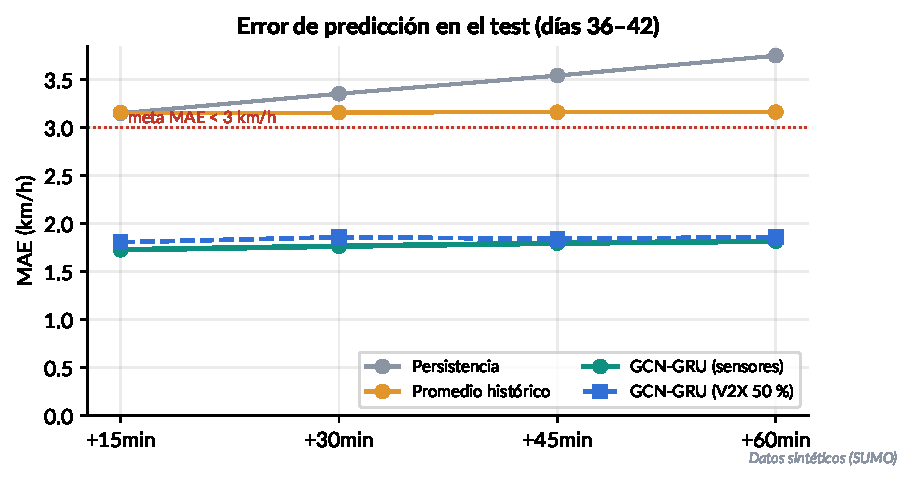
\includegraphics[width=\columnwidth]{pred_horizonte.pdf}
\caption{Error medio absoluto en el test según el horizonte \sint.}
\label{fig:horizonte}
\end{figure}

\subsection{Detección de incidentes}
La Tabla~\ref{tab:aid} resume el test y la Fig.~\ref{fig:aidazar} compara con el detector al azar. En los días con incidentes y sensores, el AID encuentra 19 de 21 incidentes con impacto en 4,5~min (intervalo de confianza del 95~\% de la DR: 69--94~\%), frente al 14~\% del azar, y cumple DR y MTTD. Con V2X la detección baja a 76~\%, porque con la mitad de los vehículos la señal por minuto es más ruidosa. En los días normales solo hay 6 incidentes con impacto; el AID encuentra 5, pero tarda 7,3~min. La FAR queda en 1,9~\% en días normales y 4,4~\% en días con 8 incidentes, dentro de la meta.

\begin{table}[t]
\centering
\caption{AID en el test con el umbral elegido sin test \sint}
\label{tab:aid}
\footnotesize
\setlength{\tabcolsep}{3.5pt}
\begin{tabular}{@{}lrrrrr@{}}
\toprule
Días, fuente & DR imp. & Azar & DR todos & FAR & MTTD \\
\midrule
36--42, sensores & 83 \% & 50 \% & 71 \% & 1,9 \% & 7,3 min \\
36--42, V2X & 83 \% & 67 \% & 65 \% & 1,9 \% & 5,0 min \\
117--120, sensores & 90 \% & 14 \% & 81 \% & 4,4 \% & 4,5 min \\
117--120, V2X & 76 \% & 52 \% & 69 \% & 4,5 \% & 2,9 min \\
\bottomrule
\end{tabular}
\end{table}

\begin{figure}[t]
\centering
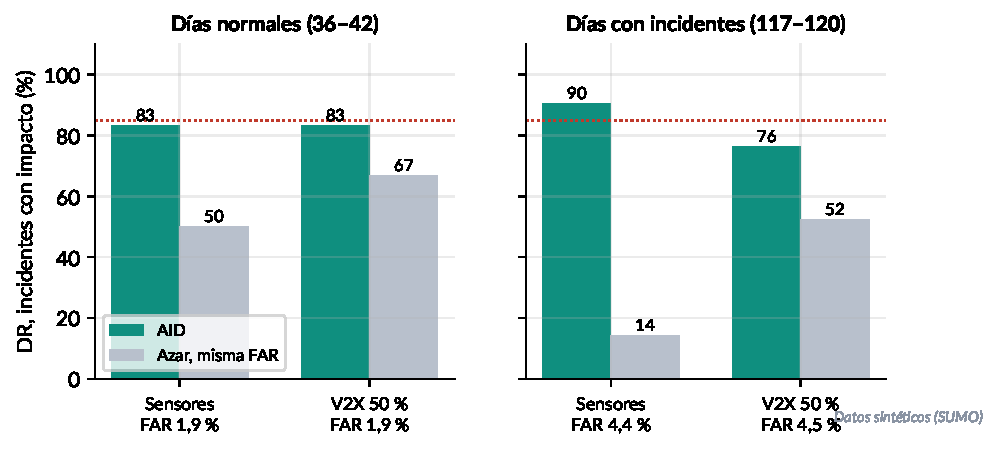
\includegraphics[width=\columnwidth]{aid_azar.pdf}
\caption{DR de los incidentes con impacto frente a un detector al azar con la misma FAR; la línea punteada es la meta de 85~\% \sint.}
\label{fig:aidazar}
\end{figure}

\subsection{Aviso V2X en bucle cerrado}
El AID en línea confirmó el cierre 2,65~min después de su inicio y se avisó a 460 vehículos, aunque 317 de esos avisos (69~\%) salieron antes del incidente por falsas alarmas; como el DENM caduca, esos vehículos volvieron a su ruta y ese costo está incluido. La Tabla~\ref{tab:sil} y la Fig.~\ref{fig:silcola} muestran el resultado sobre los 30\,700 viajes de la ventana: la demora de los afectados baja 27,8~\% y la de toda la red 8,1~\%. La cola máxima casi no cambia, porque los vehículos que ya están en el tramo no pueden salir; la ganancia está en los que todavía no llegan.

\begin{table}[t]
\centering
\caption{Bucle cerrado en SUMO, incidente \texttt{inc119\_3} \sint}
\label{tab:sil}
\footnotesize
\begin{tabular}{@{}lrrr@{}}
\toprule
Métrica & Sin IA & Con IA & Cambio \\
\midrule
Pérdida de tiempo, afectados (s) & 314 & 227 & −27,8 \% \\
Tiempo de viaje, afectados (s) & 928 & 853 & −8,1 \% \\
Pérdida media de la red (s) & 152,8 & 140,4 & −8,1 \% \\
VHT de la red (veh·h) & 5116 & 5019 & −1,9 \% \\
Cola máxima (m por carril) & 126 & 123 & −2,8 \% \\
\bottomrule
\end{tabular}
\end{table}

\begin{figure}[t]
\centering
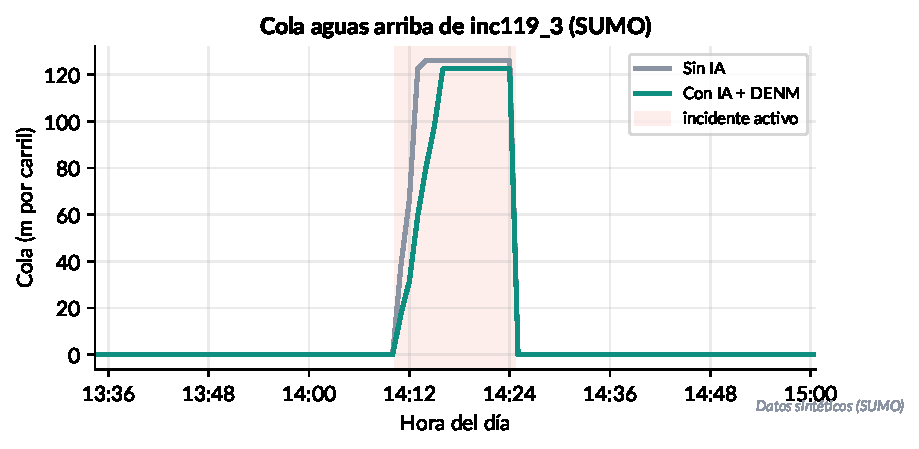
\includegraphics[width=\columnwidth]{sil_cola.pdf}
\caption{Cola aguas arriba del cierre, medida en SUMO con y sin aviso \sint.}
\label{fig:silcola}
\end{figure}

\begin{figure*}[t]
\centering
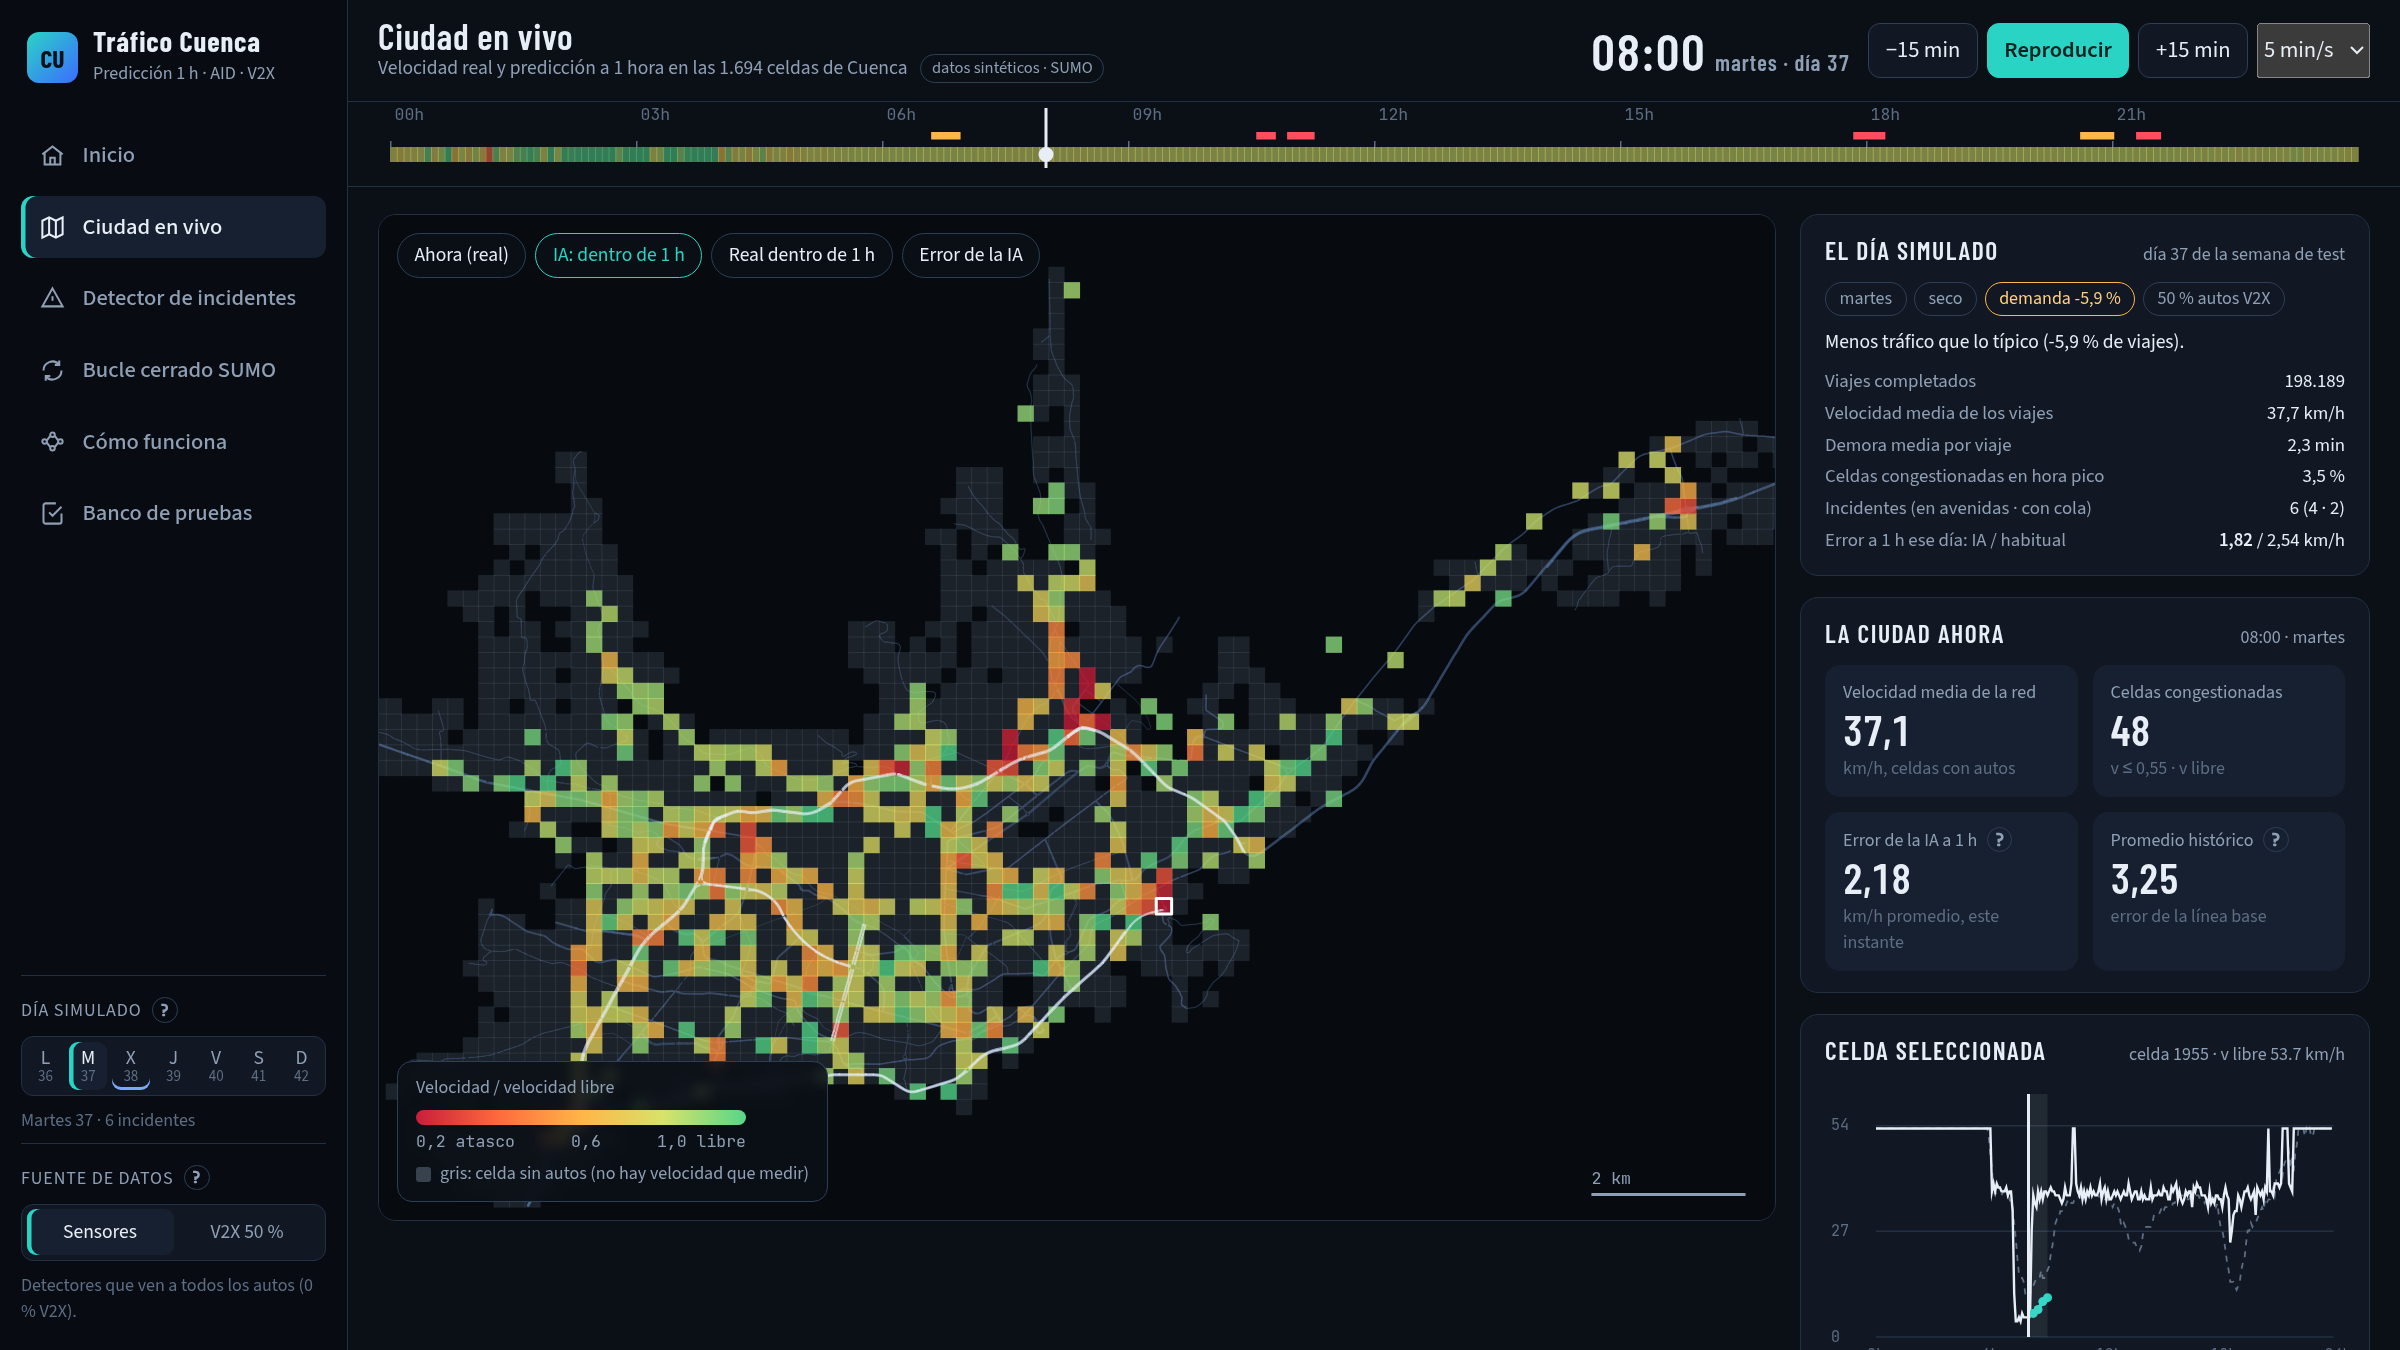
\includegraphics[width=.49\textwidth]{dash_ciudad_pred.png}\hfill
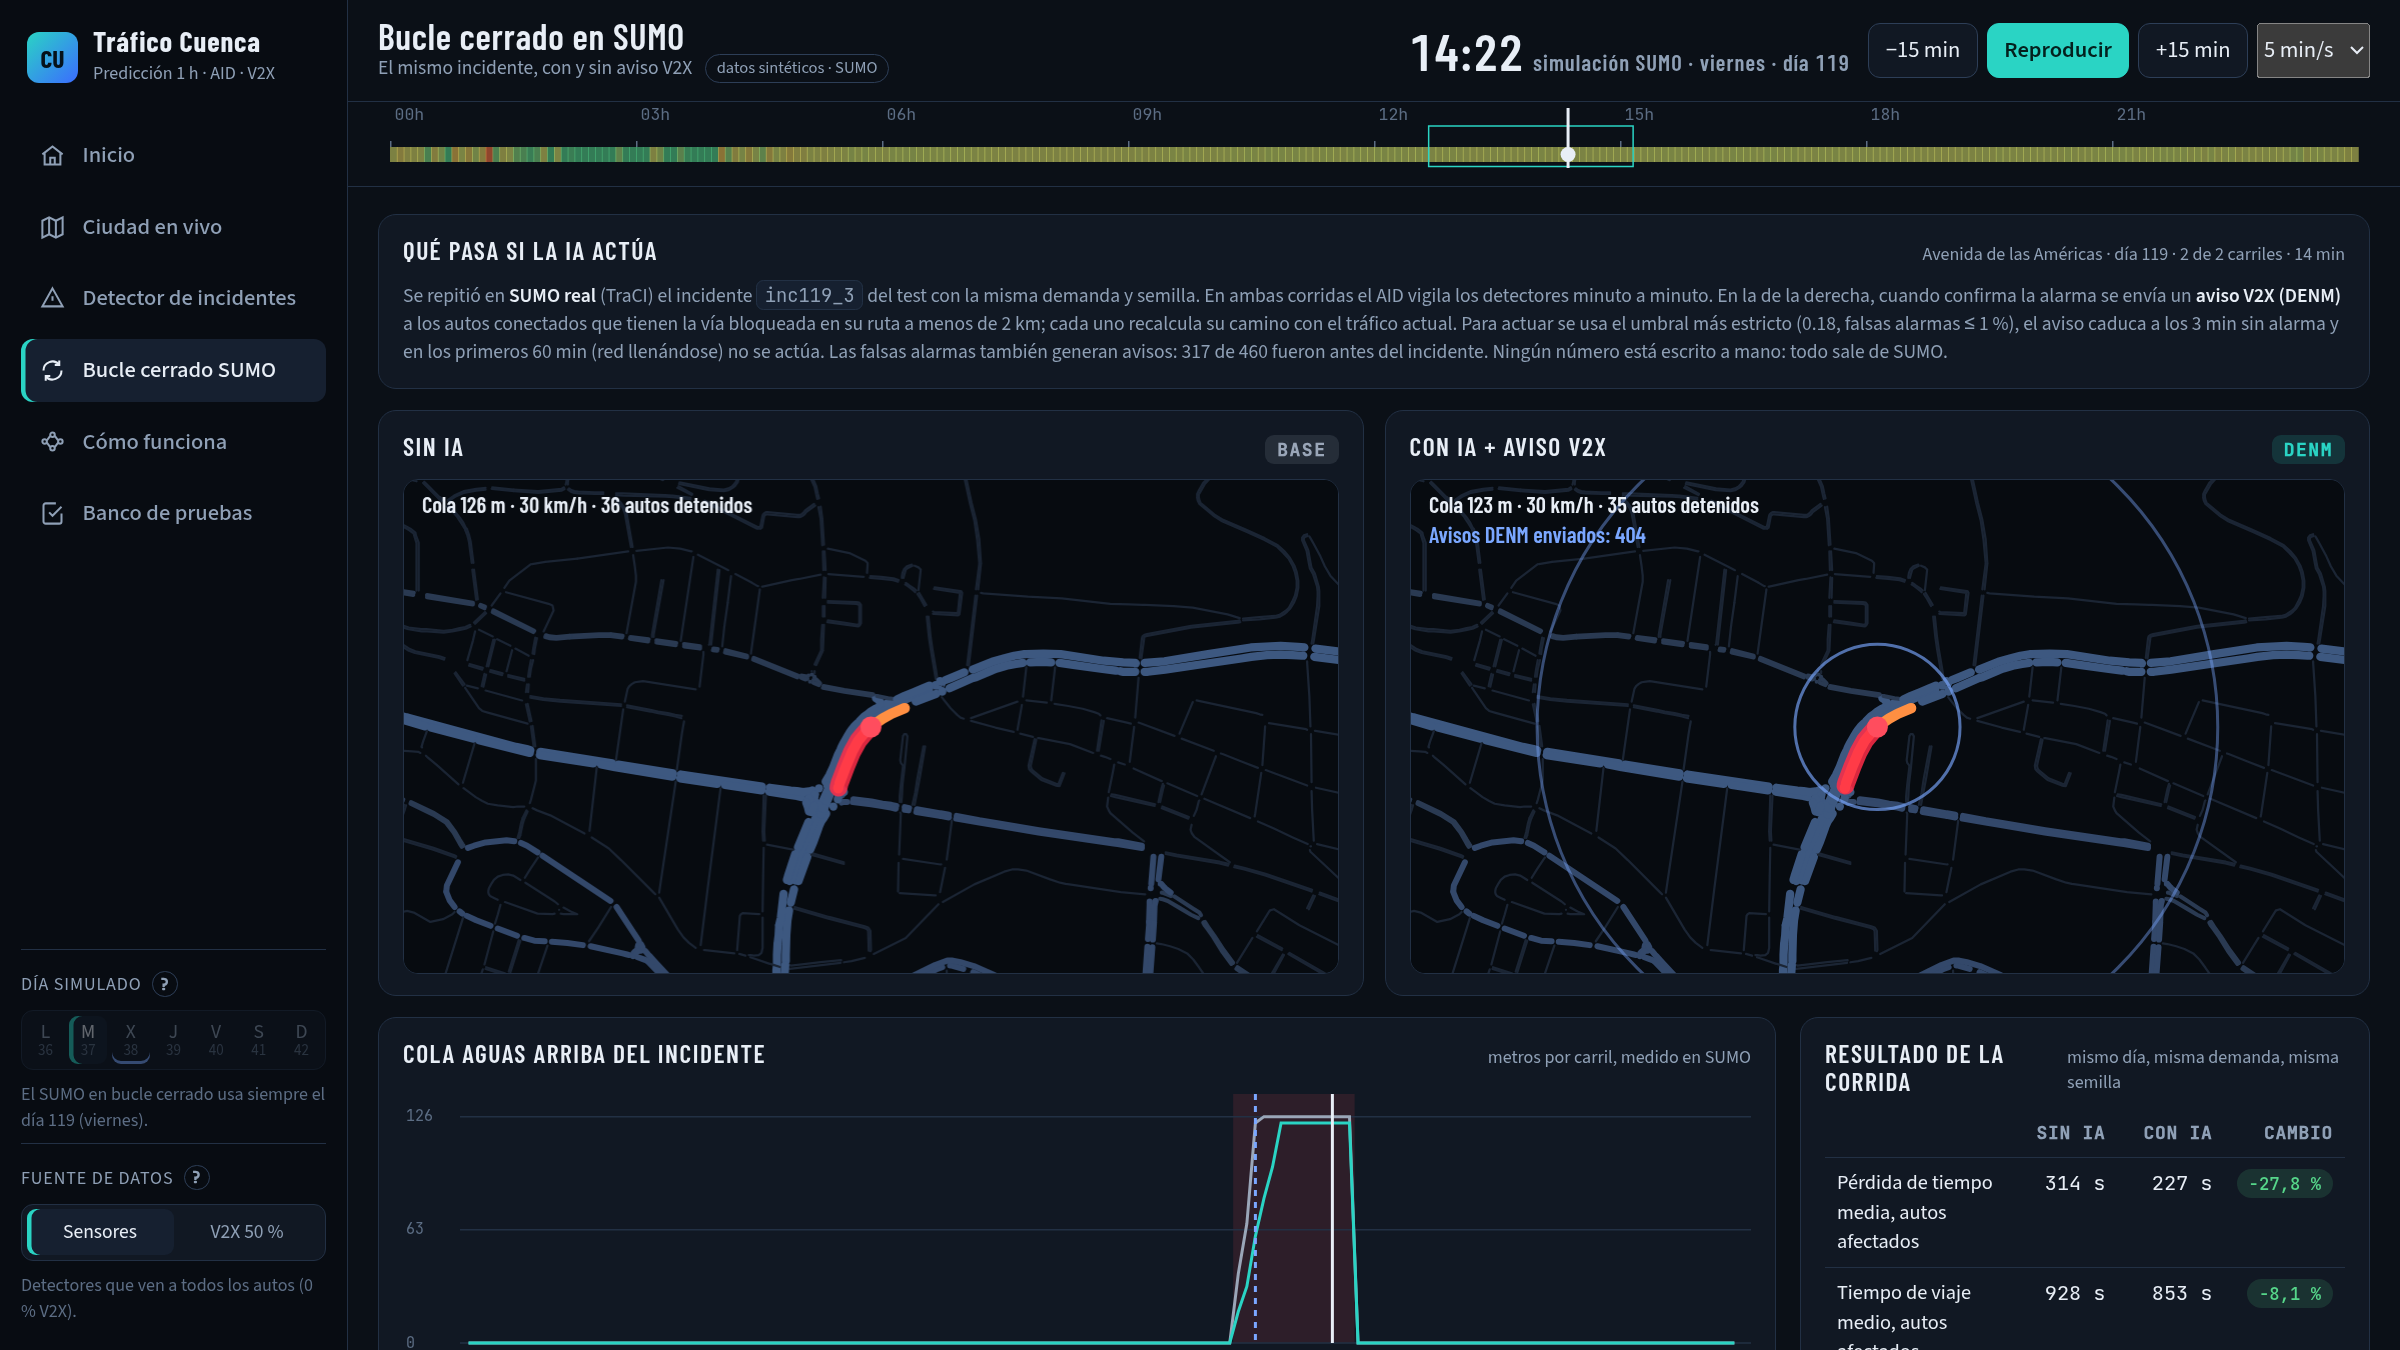
\includegraphics[width=.49\textwidth]{dash_sil.png}
\caption{Tablero interactivo \sint. Izquierda: predicción a 1~h sobre la ciudad, ficha del día y pronóstico de una celda. Derecha: bucle cerrado en SUMO con y sin aviso V2X.}
\label{fig:dash}
\end{figure*}

\section{Discusión}
\textbf{Frente al estado del arte.} Los modelos espaciotemporales de la Sección~\ref{sec:arte} se evalúan sobre autopistas con datos reales de detectores, como PeMS o METR-LA, y reportan su error como un número aislado. Nuestro MAE no es comparable en valor absoluto con esos trabajos: la red es urbana, los datos son sintéticos y el horizonte es fijo a 60~min. La diferencia está en el enfoque. Predecir la corrección sobre el promedio histórico permite un modelo de 29\,908 parámetros que gana justo donde lo habitual falla (congestión y lluvia) y que se mantiene con solo una parte de los vehículos conectados. En detección, la comparación con un detector al azar con la misma FAR es una práctica que rara vez se reporta, y muestra que una DR alta puede deberse solo a disparar muchas alarmas. En el aviso, a diferencia de los estudios que evalúan el rerouting con información perfecta, aquí la acción depende de un detector imperfecto, y su costo, los avisos por falsas alarmas, queda incluido en el resultado.

\textbf{Compromiso entre detectar y no molestar.} Bajar la FAR de 6,5 a 4,4~\% en los días cargados retrasó la detección en los días tranquilos, donde la cola se forma despacio (MTTD de 7,3~min). En el SIL se usó un umbral más estricto, y aun así el 69~\% de los avisos fueron por falsas alarmas. Que la red mejore de todos modos se debe a que los avisos caducan y el navegador solo desvía si se gana tiempo. Para un sistema operable hay que reducir esas falsas alarmas.

\textbf{Validez del dato sintético.} El gemelo digital reproduce órdenes de magnitud de Cuenca (Anexo~\ref{an:valida}), pero no su variabilidad real: no hay buses, motos, eventos especiales, fallas de sensores ni conductores que se desvíen por su cuenta. Los incidentes son vehículos detenidos con duración conocida. Por eso los resultados se presentan como sintéticos, y la cifra relevante es la mejora relativa frente a la línea base en las mismas condiciones, no el valor absoluto.

\textbf{Alcance del bucle cerrado.} El SIL evalúa un solo cierre total con una semilla. Demuestra que el mecanismo funciona, pero no basta para estimar la mejora media sobre muchos incidentes; ese es el siguiente experimento, y el script ya acepta cualquier incidente (\texttt{--inc}).


\section{Conclusiones}
El lazo completo funciona sobre el gemelo digital de Cuenca. La predicción a 1~h \ok{} con 1,82~km/h de error (1,86 con V2X al 50~\%), 43~\% menos que el promedio histórico, y se mantiene en lluvia, con más demanda y con otra penetración. El AID cumple la meta de falsas alarmas y detecta el 90~\% de los incidentes con cola en 4,5~min, seis veces más que el azar, pero todavía \no{} toda la meta: tarda 7,3~min en días normales y con V2X detecta el 76~\%. El aviso DENM reduce un 27,8~\% la demora de los afectados y un 8,1~\% la de toda la red, siempre que se limite a un área de relevancia, caduque y el navegador use tiempos actuales. Como trabajo futuro proponemos etiquetar las colas secundarias como parte del incidente, usar la predicción a 15~min como entrada del AID, probar el SIL con varios incidentes y penetraciones, y reemplazar el dato sintético por datos de la EMOV con el mismo formato.

\section{Replicabilidad del experimento}\label{sec:replica}
Todo el experimento está en el repositorio \url{\Repo}, etiqueta \texttt{\Tag}, que es la versión evaluada en este informe. El \texttt{README} basta para repetirlo en otra máquina.

\textbf{Entorno.} SUMO 1.12 en la imagen Docker \texttt{van3twin:jammy} del repositorio del curso; Python 3.13.12 con numpy 2.5.4, pandas 3.1.1, pyarrow 26.0.1, scikit-learn 1.9.1, PyTorch 2.14.1 (CPU), joblib 1.6.0, matplotlib 3.11.2 y pytest 9.2.0, fijados en \texttt{requirements.txt}. El informe se compila con \texttt{tectonic}.

\textbf{Semillas y parámetros.}
\begin{itemize}
\item Calendario de días: semilla 2026. Cada día en SUMO y \texttt{duarouter}: semilla 1000~+~día. Días extra del AID: semilla 2027. Barrido de saturación: semillas 101, 202 y 303.
\item GCN-GRU: \texttt{torch.manual\_seed(42)}, AdamW con tasa 0,002, 32 unidades ocultas, lotes de 16, 12 épocas con sensores y 8 con V2X.
\item AID: \texttt{random\_state=42}, 300 iteraciones, tasa 0,06 y 48 hojas.
\item SIL: radio de 2~km, penalización de 600~s, caducidad de 3~min y calentamiento de 60~min.
\end{itemize}
El Anexo~\ref{an:param} lista los parámetros del generador.

\textbf{Un solo script.} \texttt{./repetir\_experimento.sh} entrena y evalúa todo desde el dataset (unas 2,5~h en CPU). Con \texttt{--desde-cero} construye la red desde OSM y genera el dataset en SUMO (unas 13~h). Con \texttt{--solo-figuras} regenera en 2~min las tablas, figuras, el tablero y las pruebas desde las salidas guardadas en \texttt{v2/resultados/}. La Tabla~\ref{tab:scripts} indica qué genera cada resultado.

\begin{table}[h]
\centering
\caption{Scripts que regeneran cada tabla y figura}
\label{tab:scripts}
\scriptsize
\setlength{\tabcolsep}{2.5pt}
\begin{tabular}{@{}L{2.35cm}L{2.9cm}L{3.1cm}@{}}
\toprule
Resultado & Script & Salida \\
\midrule
Tabla~\ref{tab:pred}, Fig.~\ref{fig:horizonte} & \texttt{entrenar\_prediccion.py} & \texttt{metricas\_prediccion\_*.json} \\
Tabla~\ref{tab:aid}, Fig.~\ref{fig:aidazar} & \texttt{entrenar\_aid.py} & \texttt{metricas\_aid\_*.json} \\
Tabla~\ref{tab:sil}, Fig.~\ref{fig:silcola} & \texttt{sil\_sumo.py} & \texttt{sil\_inc119\_3\_gt.json} \\
Tabla~\ref{tab:valida} & \texttt{validar\_sintetico.py} & \texttt{validacion\_sintetico.json} \\
Figuras (PDF) & \texttt{informe/figuras\_informe.py} & \texttt{informe/figuras/} \\
Fig.~\ref{fig:dash} & \texttt{construir\_dashboard.py} & \texttt{dashboard/} \\
Conteo de pruebas & \texttt{pytest v2/pruebas} & \texttt{informe/pruebas.tex} \\
\bottomrule
\end{tabular}
\end{table}

\textbf{Datos.} El dataset completo (1,5~GB) se regenera de forma determinista con el script. El repositorio incluye la red, el OSM de origen, las tablas pequeñas del dataset y todas las salidas que respaldan las cifras.


\bibliographystyle{IEEEtran}
\bibliography{base,referencias}

\appendices
\section{Supuestos}\label{an:supuestos}
\begin{enumerate}
\item \textbf{Solo automóviles.} No hay buses, motos ni tranvía. El tranvía hacía abortar SUMO~1.12 en los cruces, y los buses no cambian la velocidad media que se predice.
\item \textbf{Comportamiento igual.} Los vehículos conectados conducen igual que los demás (modelo Krauss): estar conectado no implica conducción automatizada.
\item \textbf{Rutas fijas.} Sin el aviso, los conductores no se desvían, por recomendación del docente. En el SIL, el cambio de ruta es precisamente la intervención, y solo lo hacen los vehículos avisados.
\item \textbf{Penetración V2X fija.} Es de 50~\% en los días normales y de 30 y 70~\% en los de estrés. Los vehículos conectados son una muestra aleatoria del tráfico.
\item \textbf{Comunicación ideal.} El DENM llega sin pérdidas ni retardo a todos los vehículos V2X del área de relevancia; la cobertura de radio no se simula.
\item \textbf{Incidentes simulados.} Un incidente es un vehículo detenido por carril bloqueado. Su inicio y fin reales se toman de la salida de SUMO.
\item \textbf{Lluvia.} Se representa con más demanda y conductores más prudentes, no con un modelo de adherencia.
\item \textbf{Días independientes.} Cada día empieza con la red vacía y una hora de calentamiento que se descarta.
\end{enumerate}

\section{Parámetros del generador sintético y su fuente}\label{an:param}
La Tabla~\ref{tab:param} resume los parámetros del generador. Donde no hay una cifra publicada para Cuenca, el valor se fijó por un criterio propio que se indica (\emph{diseño}).

\begin{table}[h]
\centering
\caption{Parámetros del generador sintético}
\label{tab:param}
\scriptsize
\setlength{\tabcolsep}{2.5pt}
\begin{tabular}{@{}L{2.2cm}L{2.25cm}L{3.95cm}@{}}
\toprule
Parámetro & Valor & Fuente o criterio \\
\midrule
Red vial & OSM, 15 parroquias urbanas & OpenStreetMap; límites de OSM o Ley de Tránsito (50~km/h urbano); Américas 50/70~km/h~\cite{canafe2026irap} \\
Composición del parque & solo automóviles & 32~\% de los viajes son en vehículo privado~\cite{cazorla2026unimobility}; buses y motos fuera del alcance (Anexo~\ref{an:supuestos}) \\
Demanda pico & V0 = 17\,000 veh/h & Diseño: punto de saturación de la red (eficiencia ≥ 0,95), barrido con 3 semillas \\
Viajes por día & \textasciitilde200\,000 & Conservador frente a \textasciitilde400\,000 viajes en auto estimados (1,5~M viajes, 32~\% en auto, 1,2 personas por auto~\cite{elmercurio2026movilidad,cazorla2026unimobility,elmercurio2020carros}) \\
Perfil horario & picos 07--08, 12--14, 18--19 & Picos medidos por radar~\cite{jacome2024radar} y pico de mediodía~\cite{pena2021canaris} \\
Factor del día & 0,88--1,07 & Diseño: variabilidad entre días sin colapsar la red \\
Conducción & Krauss, σ 0,5, τ 1,0 s, speedFactor N(1; 0,1) & Valores por defecto de SUMO~\cite{sumo2026vtypes} \\
Lluvia & 20~\% de días; velocidad deseada ×0,88; demanda +4~\% & Lluvia fuerte: −6 a −9~\% de velocidad libre y −10 a −11~\% de capacidad~\cite{hranac2006weather} \\
Duración de incidentes & 10--25 min & Incidentes ``menores'' (< 30 min)~\cite{fhwa2009mutcd6i,li2018incidentduration} \\
Penetración V2X & 50~\% (30 y 70 en estrés) & Diseño: escenario intermedio y sensibilidad \\
Semillas & 1000 + día; 2026; 2027 & Reproducibilidad \\
\bottomrule
\end{tabular}
\end{table}


\section{Validación del dato sintético frente a datos reales}\label{an:valida}
Como no hay datos de la EMOV EP para el periodo, la validación compara magnitudes del dataset con cifras publicadas de Cuenca (Tabla~\ref{tab:valida}; \texttt{validar\_sintetico.py}). El volumen simulado de la Av.~de las Américas se mide como un aforo: los vehículos que cruzan una línea transversal en cada tramo de 200~m, sumando ambos sentidos, la vía central y las laterales, en los 24 laborables secos.

\begin{table}[h]
\centering
\caption{Dato sintético frente a cifras reales de Cuenca}
\label{tab:valida}
\scriptsize
\setlength{\tabcolsep}{2.5pt}
\begin{tabular}{@{}L{2.4cm}L{2.0cm}L{2.15cm}L{1.75cm}@{}}
\toprule
Magnitud & Real & Sintético \sint & Lectura \\
\midrule
Américas, hora pico & 4500--5400 veh/h~\cite{elmercurio2021americas,elmercurio2022americas} & máx. 2610 veh/h (p90 2291) & \textasciitilde50--58~\% \\
Américas, por día & 75\,000 veh~\cite{elmercurio2021americas} & máx. 34\,831 veh & \textasciitilde46~\% \\
Viajes en auto por día & \textasciitilde400\,000 (estimado) & 207\,784 & \textasciitilde52~\% \\
Hora pico mañana & 07:00--08:00~\cite{jacome2024radar} & 08:00--09:00 & 1~h de desfase \\
Hora pico tarde & 18:00--19:00~\cite{jacome2024radar} & 18:00--19:00 & coincide \\
Efecto de la lluvia & −6 a −9~\% vel. libre, −10 a −11~\% capacidad~\cite{hranac2006weather} & −14,8~\% vel. de viaje & más severo \\
Límites, Américas & 50 y 70 km/h~\cite{canafe2026irap} & 50 y 70 km/h (y otros tramos) & coincide \\
\bottomrule
\end{tabular}
\end{table}

\textbf{Lectura.} El sintético reproduce la forma del tráfico real: el pico de la tarde y, con una hora de desfase, el de la mañana; los límites de velocidad del corredor; y un efecto de la lluvia del mismo signo, algo más severo porque combina menor velocidad y más demanda. En volumen está en el orden de magnitud correcto, pero es conservador: los tres indicadores de volumen quedan en torno a la mitad de las cifras reales, que además son de prensa y sin método declarado. La demanda pico se fijó en la saturación de la red simulada sin rerouting; con más demanda la congestión no se disuelve. Por eso los resultados deben leerse como sintéticos: la mejora relativa frente a la línea base es la cifra relevante, y con demanda real el beneficio del aviso podría ser distinto. Un aforo propio en la Av. de las Américas, cargado con el formato del Anexo~\ref{an:transicion}, permitiría recalibrar la demanda.


\section{Transición al dato real}\label{an:transicion}
El código no depende del origen de los datos, sino de un formato fijo de tablas Parquet, documentado en \texttt{FORMATO\_DATOS.md}:
\begin{itemize}
\item velocidades por celda cada 5~min;
\item conteos, velocidad y ocupación por arista de corredor cada minuto;
\item calendario de días;
\item registro de incidentes.
\end{itemize}
El script \texttt{validar\_datos.py} revisa que una carpeta tenga esas tablas, columnas, tipos y rangos físicos, y la variable \texttt{RVH\_DATOS} apunta el proyecto a esa carpeta. Cuando lleguen los conteos de la EMOV EP o de una cámara, basta con convertirlos a ese formato. Los datos de una sola fuente se copian en las dos vistas (\texttt{gt} y \texttt{obs}). Ningún script de entrenamiento, evaluación o visualización cambia.


\end{document}
